\documentclass{article}
\usepackage[OT1]{fontenc}
\usepackage{graphicx}
\usepackage{setspace}
\usepackage{anysize}
\usepackage{enumerate}
\usepackage{amssymb}
\usepackage{algorithm2e}
\usepackage{amsthm}
\marginsize{3cm}{3cm}{0cm}{3cm}

\fontfamily{ptm}\fontsize{14}{14}\selectfont 
\onehalfspacing

\setlength{\parindent}{0pt}
% \setlength{\textwidth}{1.5\textwidth}

\begin{document}
\begin{center}
\textbf{\large{
HOMEWORK 1 \\
(Out: Monday, September 19, 2011; Due: Friday, October 7, 2011) \\}}
\textsc{\Large{Shumin Guo}}
\end{center}

\textbf{1.} Consider the following search problem:

\begin{figure}[ht]
  \centering
  \includegraphics[width=.7\textwidth]{hwk1-1.pdf}
\end{figure}

The states are: $A, B, C, D, E$ and $F$ . The initial state is A. The goal
state is E. The actions permit movement along directed edges (for
instance, from B, we can move to $C, D$ or $E$). Assume unit step cost.

Draw the search tree that would be produced by running each of the
search algorithms BFS, DFS and IDS on this problem. When multiple
nodes are added all at once to the fringe (or queue), assume they are
added in such a way as to be removed later from the fringe in
alphabetical order. If a goal state is reached, indicate the solution
(sequence of states) that was found and whether or not it is optimal.

For IDS, give separate answers for each choice of the depth parameter.

\sffamily\upshape\selectfont
$\blacksquare$ Please see results for three algorithms in Figure \ref{fig:ai-hwk1-1}. 
\begin{figure}[h]
  \centering 
  \includegraphics[width=\linewidth]{AI-HWK-1_1.pdf}
  \caption{Search Tree Using BFS, DFS and IDS.}
  \label{fig:ai-hwk1-1}
\end{figure}

It is easy to know that the optimal state sequence is $A-B-E$, so
although all three search algorithm can reach the goal state,
\underline{only BFS and IDS with limit=2 can achieve the optimal
  solution}. \normalfont

%% a new latex command to show the unique font for the solutions.
\newcommand{\solution}[1]{~\\ $\blacksquare$ \sffamily\upshape\selectfont #1
\normalfont ~\\~ }

\textbf{2. Exercise 3.14 in R\&N. -- page 116.} \\
3.14 Which of the following are true and which are false? Explain your
answers. \\ 
a. Depth-first search always expands at least as many nodes as A*
search with an admissible heuristic. 
\solution{Right! In fact, A* algorithm is optimally efficient for any given
  consistent heuristic, which means no other optimal algorithm is
  guaranteed to expand fewer nodes than A* algorithm. This is because
  algorithms that do not expand node with $f(n)<C^*$, where $C^*$ is
  the cost of the optimal path, run the risk of missing the optimal
  solution. }

b. $h(n) = 0$ is an admissible heuristic for the 8-puzzle. 
\solution{Right! $h(n)=0$ is guaranteed to be smaller than the actual
  cost, which can be thought as the number of steps to reach the goal
  state, it is obvious that $h(n)=0$ is the minimum non-negative step
  number to achieve the goal, so it is an admissible heuristic. }

c. A* is of no use in robotics because percepts, because states, and actions
are continuous. 
\solution{Wrong! continuous states can be abstracted into discrete
  ones, such as the path planning problem in robotics, etc..  }

d. Breadth-first search is complete even if zero step costs are
allowed. 
\solution{Right! General BFS does not take into consideration step
  costs, so as long as the search graph is finite, BFS will find the
  goal regardless of the graph type. } 

e. Assume that a rook can move on a chessboard any number of squares
in a straight line, vertically or horizontally, but cannot jump over
other pieces. Manhattan distance is an admissible heuristic for the
problem of moving the rook from square A to square B in the smallest
number of moves. 
\solution{Right! By using Manhatton distance as heuristic, all any
  move can do is move one tile one step closer to the goal, it only
  can under-estimate the cost rather than over-estimate it. }

\textbf{3. Exercise 3.15 in R\&N. You need to read 3.4.6} \\
3.15 Consider a state space where the start state is number 1 and each
state $k$ has two successors: numbers $2k$ and $2k + 1$. 

a. Draw the portion of the state space for states 1 to 15.
\solution{Please see results for three algorithms in Figure
  \ref{fig:ai-hwk1-3}.
  \begin{figure}[ht]
    \centering 
    \includegraphics[width=.5\linewidth]{AI-HWK-1_3.pdf}
    \caption{State Space for Problem. }
    \label{fig:ai-hwk1-3}
  \end{figure}
}

b. Suppose the goal state is 11. List the order in which nodes will be
visited for breadth-first search, depth-limited search with limit 3,
and iterative deepening search.
\solution{
  BFS: $1 \to 2 \to 3 \to 4 \to 5 \to 6 \to 7 \to 8 \to 9 \to 10 \to 11$ \\
  DFS: $1 \to 2 \to 4 \to 8 \to 9 \to 5 \to 10 \to 11$ \\
  Depth Limited: $1 \to 2 \to 4 \to 8 \to 9 \to 5 \to 10 \to 11$  \\
  IDS(Limit = 0): 1 \\
  IDS(Limit = 1): $1 \to 2 \to 3$  \\ 
  IDS(Limit = 2): $1 \to 2 \to 4 \to 5 \to 3 \to 6 \to 7$  \\
  IDS(Limit = 3): $1 \to 2 \to 4 \to 8 \to 9 \to 5 \to 10 \to 11 $
}

c. How well would bidirectional search work on this problem? What is
the branching factor in each direction of the bidirectional search? 
\solution{
  Forward search sequence: $1 \to \underline{2} \to 3$ \\ 
  Corresponding backward search sequence $11 \to 5 \to \underline{2}$ \\
  The process is shown in Figure \ref{fig:ai-hwk1-3c}.
  
  Branching factor for forward search: 2; \\
  Branching factor for backward search: 1.

  \begin{figure}[ht]
    \centering 
    \includegraphics[width=.5\linewidth]{AI-HWK-1_3c.pdf}
    \caption{Bidirectional Search Illustration. }
    \label{fig:ai-hwk1-3c}
  \end{figure}
}

d. Does the answer to (c) suggest a reformulation of the problem that
would allow you to solve the problem of getting from state 1 to a
given goal state with almost no search? 
\solution{
  As the branching factor for backward search is only one, which means
  no search is needed for this direction, so if we can do the search
  from goal state to the initial state, we can get the action sequence
  without any search. 
}

e. Call the action going from k to $2k$ Left, and the action going to $2k
+ 1$ Right. Can you find an algorithm that outputs the solution to this
problem without any search at all?) 
\solution{
  Please see Algorithm \ref{alg:ai-hwk1-3e}. In this algorithm, I first
  generate the value from initial value 11 to the finial value of 1, and
  push the sequence of integer values into a FILO stack, and pop all the
  elements in the stack and decide to make left turn or right turn
  according to the given rule. 
}
\begin{algorithm}[H]
  % \centering
  \KwIn{Problem Description.}
  \KwOut{Sequence of action from initial state to goal.}
  \textbf{Initial State}: Node with value 1. \\
  \textbf{Goal State}: Node with value 11. \\
  \textbf{Data Structure}: Empty FILO Stack named S. \\ 
  $State$ = 11\;
  S.push($State$)\;
  % Build queue according to parent and child relation. 
  \While{$State >$ 1} {
    \If{$State$ \% 2 $\neq$ 0 } {
      % odd number. 
      $State$ = $\frac{State - 1}{2}$\;
      S.push($State$)\;
    } \Else {
      $State$ = $\frac{State}{2}$\;
      S.push($State$)\;
    }
  }
  
  % Output action sequence. 
  \While{not S.empty()} {
    $var$ = S.pop()\;
    \If{$var$ \% 2 $\neq$ 0} {
      call Right()\; 
    } \Else {
      call Left()\;
    }
  }
  \caption{test}
  \label{alg:ai-hwk1-3e}
\end{algorithm}
\vspace{1cm}
% question 4. 
\textbf{4.} Consider the following search problem:
\begin{figure}[h]
  \centering
  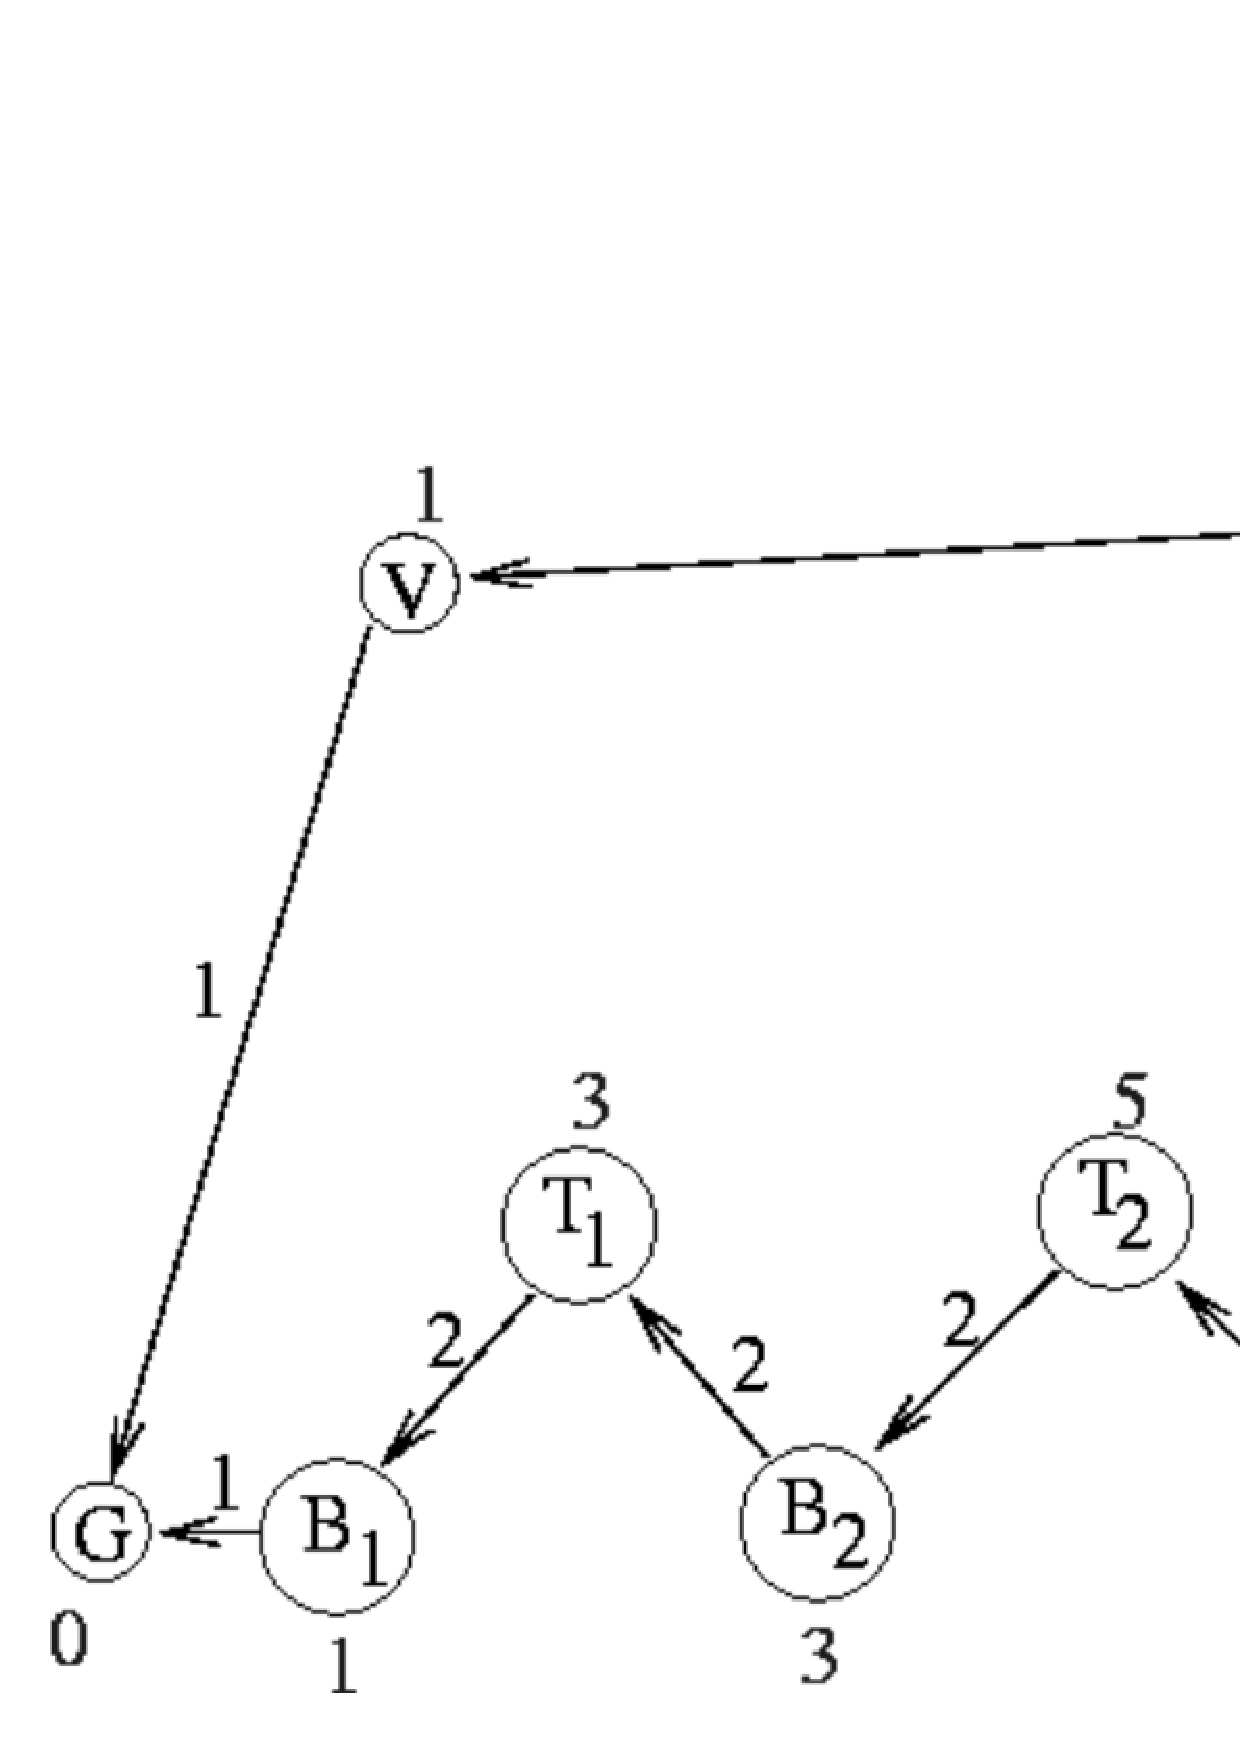
\includegraphics[width=.7\textwidth]{hwk1-2.pdf}
\end{figure}

The states are the vertices of this graph. The start state is S, and
the goal state is G. The actions permit movement along directed edges
with costs as indicated. (For instance, the cost of moving from S to U
is 2; the cost from U to V is 9.) The numbers in blue by each vertex
indicate heuristic h values. (For instance, $h(S) = 9$; $h(U) = 10$.)

a. Show that this choice of h is consistent. 
\solution{
  A heuristic $h(n)$ is consistent if for each node $n$ and its successor
  node $n^{\prime}$ generated by taking action $a$, the estimated cost
  to reach the goal from $n$ is no greater than the step cost of get
  to $n^{\prime}$ from $n$ plus the estimated cost of reaching the
  goal from $n^{\prime}$. Which can be described by the following
  in-equation, which is in the form of the general triangle inequality. 
  \[ h(n)\leq c(n,a,n^{\prime})+h(n^{\prime}) \].
  The comparison table of heuristic value of each node with its
  successor node is shown in Table \ref{tbl:ai-hwk1-4a}. As can be seen
  from the relation column of the table, the relationship between $h(n)$
  and $h(n^{\prime})+c(n,a,n^{\prime})$ is satisfied, so the choice of h
  is consistent. 
  \begin{table}[h]
    \centering
    \begin{tabular}{|l|c|c|c|c|c|c|}
      \hline
      n & $h(n)$ & $n^{\prime}$ & $c(n, a, n^{\prime})$ & $h(n^{\prime})$ &
      $c(n,a,n^{\prime})+h(n^{\prime})$ & relation \\ \hline
      S & 9 & U & 10 & 2 & 12 & $h(n)<h(n^{\prime})+c(n,a,n^{\prime})$ \\ \hline 
      U & 10 & V & 1 & 9 & 10 & $h(n)=h(n^{\prime})+c(n,a,n^{\prime})$ \\ \hline 
      V & 1 & G & 0 & 1 & 1 & $h(n)=h(n^{\prime})+c(n,a,n^{\prime})$ \\ \hline 
      S & 9 & T4 & 9 & 2 & 11 & $h(n)<h(n^{\prime})+c(n,a,n^{\prime})$ \\ \hline 
      T4 & 9 & B4 & 7 & 2 & 9 & $h(n)=h(n^{\prime})+c(n,a,n^{\prime})$ \\ \hline 
      B4 & 7 & T3 & 7 & 2 & 9 & $h(n)<h(n^{\prime})+c(n,a,n^{\prime})$ \\ \hline 
      T3 & 7 & B3 & 5 & 2 & 7 & $h(n)=h(n^{\prime})+c(n,a,n^{\prime})$ \\ \hline 
      B3 & 5 & T2 & 5 & 2 & 7 & $h(n)<h(n^{\prime})+c(n,a,n^{\prime})$ \\ \hline 
      T2 & 5 & B2 & 3 & 2 & 5 & $h(n)=h(n^{\prime})+c(n,a,n^{\prime})$ \\ \hline 
      B2 & 3 & T1 & 3 & 2 & 5 & $h(n)<h(n^{\prime})+c(n,a,n^{\prime})$ \\ \hline 
      T1 & 3 & B1 & 1 & 2 & 3 & $h(n)=h(n^{\prime})+c(n,a,n^{\prime})$ \\ \hline 
      B1 & 1 & G & 0 & 1 & 1 & $h(n)=h(n^{\prime})+c(n,a,n^{\prime})$ \\ \hline 
      G & 0 & N/A & N/A & N/A & N/A & GOAL \\ \hline 
    \end{tabular}
    \caption{Relations Table between $h(n)$ and
      $h(n^{\prime})+c(n,a,n^{\prime})$.}
    \label{tbl:ai-hwk1-4a}
  \end{table}
}

b. Draw the search tree that would result from running greedy
best-first search. Also number the nodes of the search tree in the
order in which they are expanded. For instance, place the number 1 by
the start node (associated with the start state $S$). 
\solution{
  Greedy best-first search uses the heuristic function as cost
  evaluation, which means $f(n)=h(n)$. It always tries to expand the
  node that is closest to the goal node. In general, this search
  algorithm is incomplete and not optimal. \\ 
  Please see the search tree in Figure \ref{fig:ai-hwk1-4b}. \\
  The node expand sequence is $S \to T4 \to B4 \to T3 \to B3 \to T2 \to
  B2 \to T1 \to B1 \to G$. And this sequence is also the output action
  sequence. 
  \begin{figure}[ht]
    \centering 
    \includegraphics[width=\linewidth]{AI-HWK-1_4b.pdf}
    \caption{Search Tree using Greedy Best-first Search Algorithm. }
    \label{fig:ai-hwk1-4b}
  \end{figure}
}

c. Do the same thing for $A^*$. Also indicate the g and f values
associated with each search node. 
\solution{
  A* search uses heuristic function and cost function for performance
  evaluation, so $f(n)=g(n)+h(n)$, where $g(n)$ is the cost function
  from initial node to current node, and $h(n)$ is the heuristic cost
  function from current node to the goal node. \\ 
  Please see result in Figure \ref{fig:ai-hwk1-4c}. \\
  As shown in the picture, the expand node sequence is $S \to T4 \to
  B4 \to U \to V \to G$. \\ 
  The final output sequence is $S \to U \to V \to G$. 
  \begin{figure}[ht]
    \centering 
    \includegraphics[width=\linewidth]{AI-HWK-1_4c.pdf}
    \caption{Search Tree using $A^*$ Search Algorithm. }
    \label{fig:ai-hwk1-4c}
  \end{figure}
}

% question 5. 
\textbf{5. Exercise 3.25 in R\&N. }\\
3.25 The \textbf{heuristic path algorithm (Pohl, 1977)} is a
best-first search in which the evaluation function is ,$f(n) = (2 -
w)g(n) + wh(n)$. For what values of $w$ is this complete? For what
values is it optimal, assuming that h is admissible? What kind of
search does this perform for $w = 0, w = 1$, and $w = 2$? 
\solution{
  First, we need to make sure $2-w \geq 0$ and $w \geq 0$, from this we
  can get $0\leq w \leq 2$. \\
  When $w=0$, we have $f(n)=2g(n)$, which is uniform cost search (the
  multiplier 2 will not affect the search strategy of expanding the node
  with minimum cost from initial state to current node, this idea
  applies similarly to the statements below), it is complete, in case of
  finite branching factor. As there will be a finite number of expansions
  required before the total path cost is equal to the path cost of the
  goal state. And similarly, we can show that it is also optimal. \\
  When $0 < w < 2$, the search is $A^*$ or variant of $A^*$ search,
  which is complete and optimal, in case h(n) is optimal (and actually,
  another constraint is that $wh(n) \leq h^*(n)$ for the satisfying $w$,
  here $h^*(n)$ is the optimal huristic, which is actually the minimum
  cost from initial state to goal state. But here, because $h^*(n)$ is
  not given, I simply assume this requirement is satisfied). \\
  When $w=2$, $f(n)=2h(n)$, the search becomes greedy best first search,
  which is complete in case it can keep track of all visited states. But
  it is not optimal. \\
  
  \underline{Summarizing the analysis above, we know that $f(n)$ is
    complete when $0\leq w \leq 2$.} \\
  \underline{$f(n)$ is complete when $0\leq w < 2$.}\\
  
  When $w=0$, $f(n)=(2-0)g(n)+0\times h(n) = 2g(n)$, the search will
  become uniform cost search, and if the cost step costs are equal, it
  will behave similarly to BFS. \\ 
  When $w=1$, $f(n)=(2-1)g(n)+1\times h(n) = g(n) + h(n)$, the search
  will become $A^*$ search. \\ 
  When $w=2$, $f(n)=(2-2)g(n)+2\times h(n) = 2h(n)$, the search will
  become greedy best-first search. 
}

\textbf{6. Exercise 3.26 in R\&N. } \\
3.26 Consider the unbounded version of the regular 2D grid shown in
Figure 3.9. The start state is at the origin, $(0,0)$, and the goal
state is at $(x,y)$. 

a.What is the branching factor b in this state space? 
\solution{
Branching factor for the origin point is 4. And for other points, the
branching factor is 3, so the average branching factor is
approximately 3. 
}

b.How many distinct states are there at depth k (for $k > 0$)? 
\solution{
  Number of states of depth k is $S(k) = 4\times 3^{k-1}$. 
  \begin{proof}
    When $k = 1$, $S(k) = 4\times 3^{1-1} = 4\times 1 = 4$. \\ 
    When $k = 2$, $S(k) = 4 \times 3$ \\
    Suppose the number of states for depth $k$ is $S(k) = 4\times
    3^{k-1}$, we have, when depth is $k+1$, the number of states is $3
    \times S(k) = 3\times 4 \times 3^{k-1} = 4\times 3^{k}$. 
  \end{proof}
}
c.What is the maximum number of nodes expanded by breadth-first tree
search? 
\solution{
  The complexity of BFS is denoted as $O(b^{d+1})$, by replacing b
  with 3 and replacing d with k, the complexity becomes
  $O(3^{k+1})$. Thus the number of nodes expanded is $3^{k+1}$. 
}

d.What is the maximum number of nodes expanded by breadth-first graph
search? 
\solution{
  The graph version of BFS is the same as the tree version BFS except
  that we need to keep track of all visited nodes to avoid loops, so
  the number of expanded node is also $3^{k+1}$, where k is the depth
  of the goal. 
}

e. Is $h=|u-x|+|v-y|$ an admissible heuristic for a state at (u, v)?
Explain. 
\solution{
  Yes, $h$ is an admissible heuristic. Acutually, becasue of the fact
  of the problem, an agent can only move along vertical or horizontal
  axis from the origin to the goal point. So the optimal heuristic
  will be $h^*(n)=|u-x|+|v-y|$, which means $h=h^*$ and thus $h\leq
  h^*$, so according to the property of admissible heuristic,
  $h=|u-x|+|v-y|$ is an admissible heuristic. 
}

f. How many nodes are expanded by A* graph search using h? 
\solution{
  Number of nodes expanded by $A^*$ using $h=|u-x|+|v-y|$ is
  $|u-x|+|v-y|$, which is the optimal solution to the problem. 
}

g. Does $h$ remain admissible if some links are removed? 
\solution{
  Yes, $h$ is still admissible, because by removing links from the
  graph, the fact that $h\leq h^*$ will not change. 
}

h. Does h remain admissible if some links are added between
nonadjacent states? 
\solution{
  h might become no long admissible when links are added between
  nonadjacent nodes, because the requirement $h\leq h^*$ might not be
  satisfied any more. 
}

\textbf{7. Exercise 3.27 in R\&N.} \\
$n$ vehicles occupy squares $(1, 1)$ through $(n, 1)$ (i.e., the
bottom row) of an $n \times n$ grid.  The vehicles must be moved to
the top row but in reverse order; so the vehicle i that starts in $(i,
1)$ must end up in $(n - i + 1, n)$. On each time step, every one of
the 11 vehicles can move one square up, down, left, or right, or stay
put; but if a vehicle stays put. one other adjacent vehicle (but not
more than one) can hop over it. Two vehicles cannot occupy the same
square. \\
a. Calculate the size of the state space as a function of $n$. 
\solution{
  The state space is about $n^2$. 
  \begin{proof}
    Let's consider the worst case, when n vehicles move one by one,
    which means vehicle $i$ move frist from its initial state to its
    goal state, the search space for this vehicle is roughly $n$, so
    for $n$ vehicles the total space will be roughly $n^2$. 
  \end{proof}
  This proof gives the upper bound of the state space which is second
  order polynomial. 
}

b. Calculate the branching factor as a function of n. 
\solution{
  As at each time, each vehicle has five possible actions, so the
  branching factor is $\approx 5$. 
}

c. Suppose that vehicle i is at $(x_i, y_i)$: write a nontrivial
admissible heuristic $h_i$, for the number of moves it will require to
get to its goal location ($n - i + 1$, n), assuming no other vehicles
are on the grid.
\solution{
  A heuristic function $h(i)=|n-x_i-i+1| + |n-y_i|$, which is
  admissible because the actual path cost is equal to this heuristic
  cost. So it is also an optimal cost function. 
}

d. Which of the following heuristics are admissible for the problem of
moving all n vehicles to their destinations? Explain. 
\begin{enumerate}[(i)]
\item $\sum_{i=1}^nh_i$; 
\item $max\{h_1,\ldots,h_n\}$; 
\item $min\{h_1,\ldots,h_n\}$.
\end{enumerate}
\solution{
  $(iii)$ is admissible, because it is no larger than the actual optimal
  cost. 
}

\textbf{8. Exercise 5.8. Page-197} \\
5.8 Consider the two-player game described in Figure 5.17. \\
a. Draw the complete game tree, using the following conventions:
\begin{itemize}
  \item Write each state as ($S_A, S_B$), where $S_A$ and $S_B$ denote
    the token locations. 
  \item Put each terminal state in a square box and write its game
    value in a circle. 
  \item Put loop states (states that already appear on the path to the
    root) in double square boxes. Since their value is unclear,
    annotate each with a "?" in a circle. 
\end{itemize}
\solution{
  Please see game tree in Figure \ref{fig:ai-hwk1-8a}. 
  \begin{figure}[h]
    \centering 
    \includegraphics[width=\linewidth]{AI-HWK-1_8a.pdf}
    \caption{Game tree for the two player game. }
    \label{fig:ai-hwk1-8a}
  \end{figure}
}

b. Now mark each node with its backed-up minimax value (also in a
circle). Explain how you handled the "?" values and why. 
\solution{
  The "?" values are handled by assuming that an agent with a choice
  between winning the game and entering a "?" state will always choose
  the win. That is, $min(–1,?)$ is –1 and $max(+1,?)$ is +1. If all
  successors are "?", the backed-up value is "?".
}

c. Explain why the standard minimax algorithm would fail on this game
tree and briefly sketch how you might fix it, drawing on your answer
to (b). Does your modified algorithm give optimal decisions for all
games with loops? 
\solution{
  Standard minimax is depth-first and would go into an infinite loop. It
  can be fixed by comparing the current state against the stack; and if
  the state is repeated, then return a “?” value. Propagation of “?”
  values is handled as above. Although it works in this case, it does
  not always work because it is not clear how to compare “?” with a
  drawn position; nor is it clear how to handle the comparison when
  there are wins of different degrees (as in backgammon). Finally, in
  games with chance nodes, it is unclear how to compute the average of a
  number and a “?”. Note that it is not correct to treat repeated states
  automatically as drawn positions; in this example, both (1,4) and
  (2,4) repeat in the tree but they are won positions.

  What is really happening is that each state has a well-defined but
  initially unknown value. These unknown values are related by the
  minimax equation at the bottom of page 163. If the game tree is
  acyclic, then the minimax algorithm solves these equations by
  propagating from the leaves. If the game tree has cycles, then a
  dynamic programming method must be used, as explained in Chapter
  17. (Exercise 17.8 studies this problem in particular.) These
  algorithms can determine whether each node has a well-determined value
  (as in this example) or is really an infinite loop in that both
  players prefer to stay in the loop (or have no choice). In such a
  case, the rules of the game will need to define the value (otherwise
  the game will never end). In chess, for eaxmple, a state that occurs 3
  times (and hence is assumed to be desirable for both players) is a
  draw.
}

d. This 4-square game can be generalized to n. squares for any $n >
2$. Prove that A wins if n is even and loss if it is odd. \\
\sffamily\slshape\bfseries\selectfont{Note: This solution was from the
  internet, and this note is to pay tribute to the original author of this
  solution. I copied this solution only to learn rather than ..., so,
  no credit can be given to me for this question.}\normalfont
\solution{
  This question is a little tricky. One approach is a proof by induction
  on the size of the is a loss for A and the base case $n=3$ is a win
  for game. Clearly, the base case $n=4$, the initial moves are the
  same: A and B both move one step towards A. For any $n>4$ on the each
  other. Now, we can see that they are engaged in a subgame of size
  $n-2$ on the squares $[2,\ldots,n-1]$, except that there is an extra
  choice of moves on squares 2 and $n-1$. Ignoring this for a moment, it
  is clear that if the $n-2$ is won for A, then A gets to the square
  $n-1$ before B gets to square 2 (by the definition of winning) and
  therefore gets to $n$ before B gets to 1, hence the $n$ game is won
  for A. By the same line of reasoning, if $n-2$ is won for B then $n$
  is won for B. Now, the presence of the extra moves complicates the
  issue, but not too much. First, the player who is slated to win the
  subgame $[2,\ldots,n-1]$ never moves back to his home square. If the
  player slated to lose the subgame does so, then it is easy to show
  that he is bound to lose the game itself, the other player simply
  moves forward and a subgame of size $n-2k$ played one step closer to
  the loser’s home square.
}


\textbf{9. Exercise 17.17 in R\&N. Page 691.} \\
17.17 In the children's game of rock-paper-scissors each player
reveals at the same time a choice of rock, paper, or scissors. Paper
wraps rock, rock blunts scissors, and scissors cut paper. In the
extended version rock-paper-scissors—fire-water, fire beats rock,
paper, and scissors; rock, paper, and scissors beat water; and water
beats fire. Write out the payoff matrix and find a mixed-strategy
solution to this game.
\solution{
  Let's suppose there are two players, denoted as A and B
  respectively. Please see the payoff matrix in Table
  \ref{tbl:ai-hwk1-9a}. (A is row B is column, and the matrix is in the
  form (A, B), if A beats B, value is (1, -1), if tie value is (0, 0)
  and if B beats A, value is (-1, 1)). 
  \begin{table}[h]
    \centering
    \begin{tabular}{|l|c|c|c|c|c|}
      \hline
      (A,B) & rock & paper & scissors & fire & water \\ \hline
      rock & $(0,0)$ & $ (-1,1) $  & $ (1,-1) $  &  $ (-1,1) $ &  $ (1,-1) $ \\ \hline 
      paper & $ (1,-1) $ & $(0,0)$ & $ (-1,1) $  &  $ (-1,1) $ &  $ (1,-1) $ \\ \hline
      scissors & $ (-1,1) $ & $ (1,-1) $  & $(0,0)$ &  $ (-1,1) $ & $ (1,-1) $ \\ \hline 
      fire & $ (1,-1) $ & $ (1,-1) $  & $ (1,-1) $  & $(0,0)$ &  $ (-1,1) $ \\ \hline
      water & $ (-1,1) $ & $ (-1,1) $  & $ (-1,1) $  &  $ (1,-1) $ & $(0,0)$ \\ \hline
    \end{tabular}
    \caption{Payoff matrix for rock-paper-scissors—fire-water game.}
    \label{tbl:ai-hwk1-9a}
  \end{table}

  Finding the mixed strategy solution for the game. \\ 
  Suppose the strategy profile of player A is as follows: \\ 
  A: [p1:rock; p2:paper; p3:scissors; p4:fire; p5:water], where $p1 +
  p2 + p3 + p4 + p5 = 1$. \\ 
  And the payoff matrix for player A with player B makes different
  choices can be see at Table \ref{tbl:ai-hwk1-9b}.

  \begin{table}[h]
    \centering
    \begin{tabular}{|l|l|}
      \hline
      \textbf{B plays} & \textbf{payoff} \\ \hline
      rock & $P_{rock}=p2-p3+p4-p5$ \\ \hline
      paper & $P_{paper}=-p1+p3+p4-p5$ \\ \hline
      scissors & $P_{scissors}=p1-p2+p4-p5$ \\ \hline
      fire & $P_{fire}=-p1-p2-p3+p5$ \\ \hline
      water & $P_{water}=p1+p2+p3-p4$\\ \hline
    \end{tabular}
    \caption{Payoff matrix of player A with player B has different plays.}
    \label{tbl:ai-hwk1-9b}
  \end{table} 

  We can get the solution as follows: $p1=p2=p3=\frac{1}{9}; p4=p5
  =\frac{1}{3}$. And because of the symmatric property, player B
  should have the same mixed strategy.}

\textbf{10. Exercise 17.18 in R\&N. } \\
17.18 The following payoff matrix, from Blinder (1983) by way of
Bernstein (1996), shows a game between politicians and the Federal
Reserve. 

\begin{table}[ht]
\centering
\begin{tabular}{|l|c|c|c|}
  \hline
  & Fed: contract & Fed: do nothing & Fed: expand \\ \hline
  Pol: contract & F = 7, P = 1 & F = 9, P = 4 & F = 6, P = 6 \\ \hline
  Pol: do nothing & F = 8, P = 2 & F = 5, P = 5 & F = 4, P = 9 \\ \hline
  Poi: expand & F = 3, P = 3 & F = 2, P = 7 & F = 1, P = 8 \\ \hline
\end{tabular}
\end{table}

Politicians can expand or contract fiscal policy, while the Fed can
expand or contract monetary policy. (And of course either side can
choose to do nothing.) Each side also has preferences for who should
do what neither side wants to look like the bad guys. The payoffs
shown are simply the rank orderings: 9 for first choice through 1 for
last choice. Find the Nash equilibrium of the game use pure
strategies. Is this a Pareto-optimal solution? You might wish to
analyze the policies of recent administrations in this light.
\solution{
  There is only one nash equilibrium when $F=6, P=6$. \\
  It is not Pareto-optimal.
}


\textbf{11. (This is for graduate students only) Exercise 3.4 in
  R\&N.} \\
3.4 Show that the 8-puzzle states are divided into two disjoint sets,
such that any state is reachable from any other state in the same set,
while no state is reachable from any state in the other
set. \textbf{(Hint: See Berlekamp et al. (1982).)} Devise a procedure 
to decide which set a given state is in, and explain why this is
useful for generating random states. 
\solution{
  First, let's take a look at Figure \ref{fig:ai-hwk1-11}. In this
  figure we define a counting as follows: as the arrow in the figure
  shows, we count the number of tiles that are smaller than current
  number for each value. In this example the number is 1 for 2, 6 for 8,
  1 for 3, 0 for 1, 2 for 6, 0 for 4, 1 for 7, 0 for 5. And by summing
  up the number we get $sum = 1+6+1+0+2+0+1+0 = 11$. And it is obvious
  that for a random initial state, $sum$ will either be an \textbf{odd}
  number or and \textbf{even} number.

  And for each non-goal state, the blank tile has two possible
  actions, move along the row and move along the column. When the blank
  tile moves along the row of the board, it is trival to prove that
  the number $sum$ will not change. While when the blank tile moves
  along the column, the number sequence permutation will only change
  the number $sum$ by $\{-2, 0, 2\}$ which will not change the parity
  of $sum$, that is if $sum$ is \textbf{odd} before the move, it will
  still be \textbf{odd} after the move, and similarly for
  \textbf{even}. This tells us that the parity property of the
  8-puzzle problem will be constant during the game playing process. 

  And according to the description above, the 8-puzzle state will be
  divided into two disjoint sets, names \textbf{odd} set and
  \textbf{even} set. The game will be solvable if the initial state is
  in the same set as the goal state, and will not be solvable
  otherwise. 

  The seperation of states tells us that in order to generate a random
  state for the 8-puzzle game, we need to make sure it is in the same
  set as the goal state. 
}
\begin{figure}[h]
  \centering 
  \includegraphics[scale=.5]{AI-HWK-1_11.pdf}
  \caption{Counting illustration for 8-puzzle game. }
  \label{fig:ai-hwk1-11}
\end{figure}

\textbf{12. (This is for graduate students only) Exercise 3.29 in
  R\&N.} \\
3.29 Prove that if a heuristic is consistent, it must be admissible.
Construct an admissible heuristic that is not consistent.
\solution{
  A heuristic $h(n)$ is consistent if for each node nand its successor
  node $n^{\prime}$ generated by taking action $a$, the estimated cost to reach the
  goal from $n$ is no greater than the step cost of get to $n^{\prime}$ from nplus
  the estimated cost of reaching the goal from $n^{\prime}$. Which can be
  describe by the following in-equation. This is in the form of the
  general triangle inequality. 
  \[ h(n) \leq c(n, a, n^{\prime}) + h(n^{\prime}) \]
  where $c(n, a, n^{\prime})$ is the step cost of getting to
  $n^{\prime}$ by taking action $a$ at $n$. 

  1), Prove when a heuristic is consistent it must be admissible.
  
  \begin{proof}
    Let $k(n)$ be the cost of the cheapest path from n to the goal node. We will
    proove by induction on the number of steps to the goal that $h(n)
    \leq k(n)$. \\
    1, when n is a goal, there is 0 step to the goal, therefore $h(n)
    = 0 \leq k(n)$. \\
    2, If $n$ is $i$ steps away from the goal, there must exist some
    successor $n^{\prime}$ of n generated by some action $a$ such that
    $n^{\prime}$ is on the optimal path from $n$ to the goal (via action
    $a$) and $n^{\prime}$ is $i - 1$ steps away from the goal. Therefore,
    \[ h(n) \leq c(n, a, n^{\prime}) + h(n^{\prime}) \] But by the
    induction hypothesis, \[ h(n^{\prime}) \leq
    k(n^{\prime}) \]. Therefore, \[ h(n) \leq c(n, a, n^{\prime}) +
    k(n^{\prime}) = k(n) \] since $n^{\prime}$ is on the optimal path from
    $n$ to the goal via action $a$.
    
  \end{proof}
  This proves the first statement. \\

  2), Construct an admissible heuristic for some search problem, that
  is not consistent. \\
  Consider a search problem where the states are nodes along a path $P
  = n_0, n_1, . . . , n_m$ where $n_0$ is the start state, $n_m$ is the
  goal state and there is one action from each state $n_i$ which gives
  $n_{i+1}$ as a successor with cost 1. The cheapest cost to the goal
  from a state $i$ is then $k(n_i) = m - i$. Define a heuristic function
  as follows: \[ h(n_i)=m-2\lceil i/2 \rceil \] for all states $n_i,
  h(n_i)\leq k(i)$, and so $h$ is admissible. However, if $i$ is odd,
  then $h(n_i)=h(n_{i+1})>1+h(n_{i+1})$. Thus $h$ is not consistent.
}
\end{document}